\subsection{Advanced Momentum and Variance Reduction (2024--2025)}
\paragraph{Adan (Adaptive Nesterov Momentum).}
\begin{figure}[H]
\centering
\fitfigure{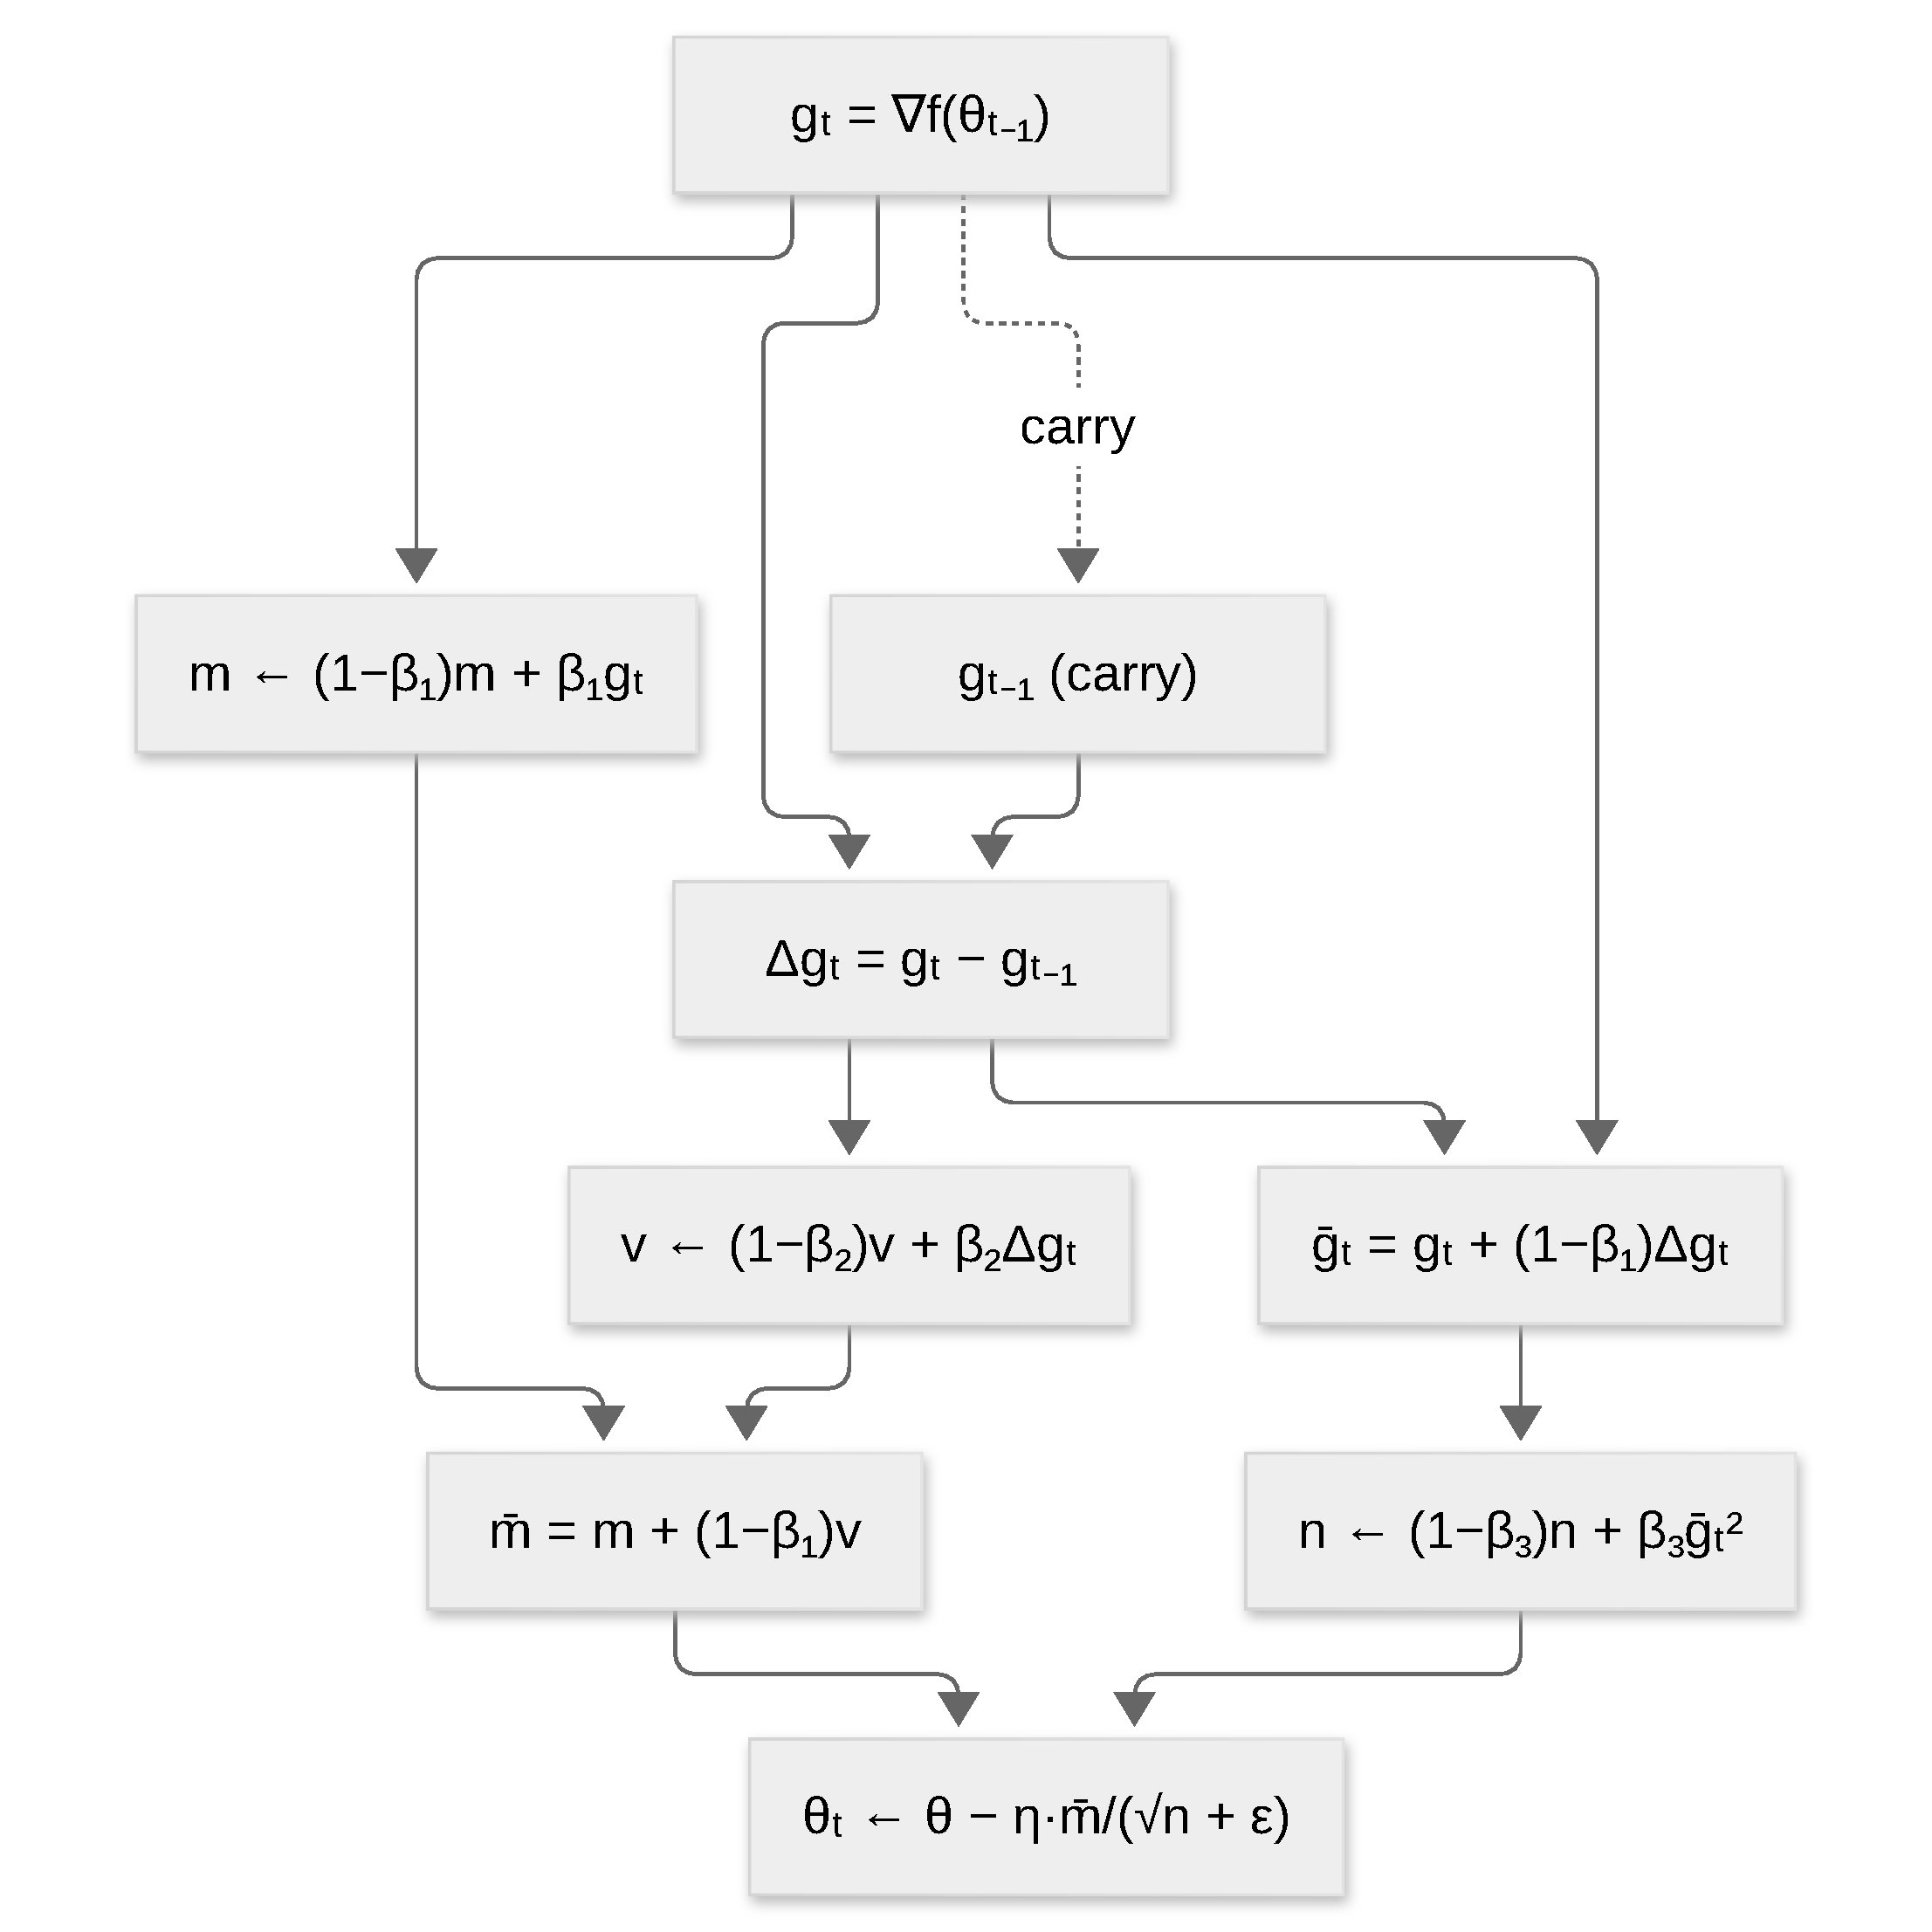
\includegraphics{figures/optimizers/adan.pdf}}
\caption{Step flow of Adan: Nesterov momentum estimation from the gradient difference, with three state buffers and a combined momentum step.}
\label{fig:opt-adan}
\end{figure}
Adan reformulates Nesterov acceleration without the extra gradient computation required by classical Nesterov SGD. The algorithm maintains three momentum buffers:
\begin{align}
m_t &= (1-\beta_1)m_{t-1} + \beta_1 g_t \quad\text{(first moment)} \\
v_t &= (1-\beta_2)v_{t-1} + \beta_2(g_t - g_{t-1}) \quad\text{(velocity/gradient difference)} \\
n_t &= (1-\beta_3)n_{t-1} + \beta_3[g_t + (1-\beta_1)(g_t-g_{t-1})]^2 \quad\text{(Nesterov second moment)}
\end{align}
The \textbf{Nesterov Momentum Estimation} (NME) term $\bar{g}_t = g_t + (1-\beta_1)(g_t-g_{t-1})$ estimates the gradient at a future position without evaluating it. The update combines momentum with velocity:
\[\bar{m}_t = m_t + (1-\beta_1)v_t, \quad \theta_{t+1} = \theta_t - \eta\frac{\bar{m}_t}{\sqrt{n_t}+\epsilon}\]

\begin{algorithm}[H]
\caption{Adan (Adaptive Nesterov Momentum)}
\label{alg:adan}
\begin{algorithmic}[1]
\Require Initial parameters $\theta_0$, learning rate $\eta$, $\beta_1, \beta_2, \beta_3 \in (0,1)$
\Ensure Updated parameters $\theta_T$
\State Initialize: $m \gets 0$, $v \gets 0$, $n \gets 0$, $g_{-1} \gets 0$ (previous gradient)
\For{$t = 1, 2, \ldots, T$}
    \State $g_t \gets \nabla f(\theta_{t-1})$
    \State $m \gets (1-\beta_1) m + \beta_1 g_t$
    \State $\Delta g_t \gets g_t - g_{t-1}$
    \State $v \gets (1-\beta_2) v + \beta_2 \Delta g_t$
    \State Nesterov estimation: $\bar{g}_t \gets g_t + (1-\beta_1) \Delta g_t$
    \State $n \gets (1-\beta_3) n + \beta_3 \bar{g}_t^2$
    \State Combined momentum: $\bar{m} \gets m + (1-\beta_1) v$
    \State $\theta_t \gets \theta_{t-1} - \eta (\bar{m} / (\sqrt{n} + \epsilon))$
    \State $g_{t-1} \gets g_t$
\EndFor
\Return $\theta_T$
\end{algorithmic}
\end{algorithm}

\paragraph{Cons.}
\begin{itemize}[leftmargin=*]
\item Three momentum-like buffers increase memory overhead relative to Adam.
\item Additional gradient-difference bookkeeping per step.
\end{itemize}

\paragraph{Pros.}
\begin{itemize}[leftmargin=*]
\item Nesterov-style acceleration without an extra gradient evaluation.
\item Fast convergence across diverse architectures (CNNs, GANs, transformers).
\end{itemize}

\paragraph{ADOPT (Adam with Optimal Pruned Tuning).}
\begin{figure}[H]
\centering
\fitfigure{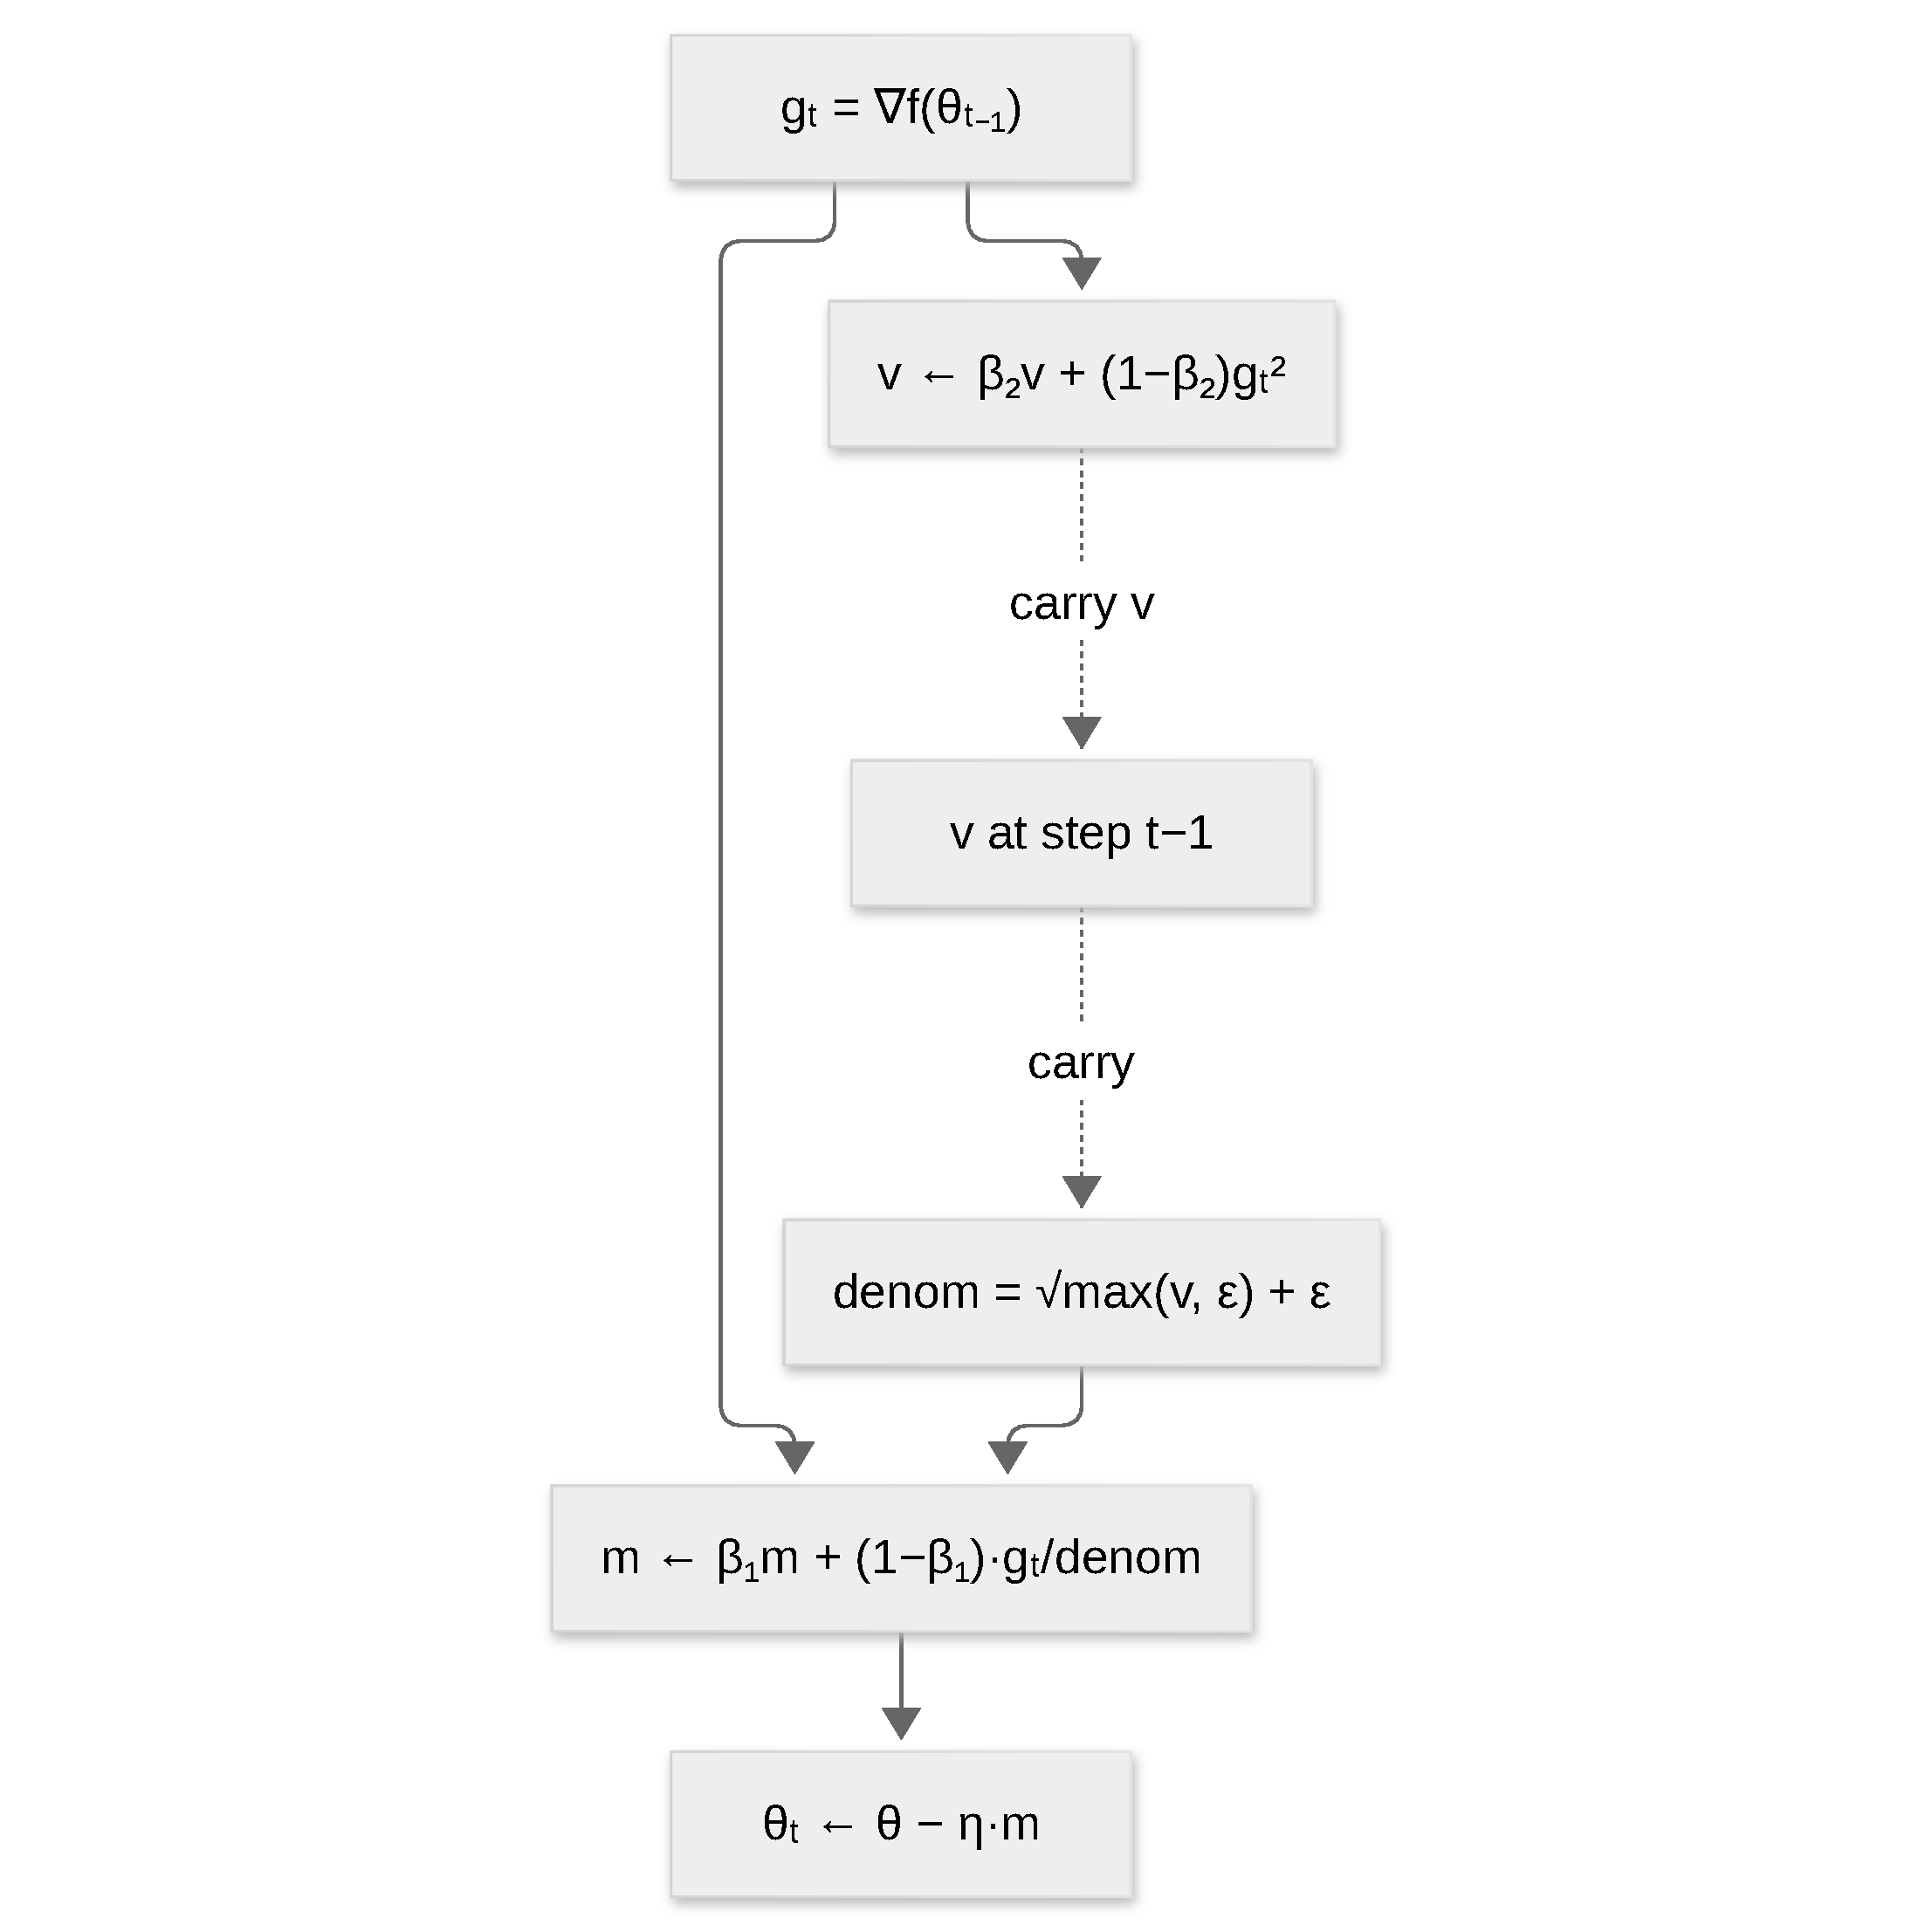
\includegraphics{figures/optimizers/adopt.pdf}}
\caption{Step flow of ADOPT: the second moment from the previous step normalizes the current gradient before the first-moment update.}
\label{fig:opt-adopt}
\end{figure}
ADOPT fixes a fundamental theoretical issue in Adam: the gradient appears in both the first moment and second moment estimates, creating circularity. ADOPT \textbf{decouples} by using the previous step's second moment for the denominator:
\begin{align}
v_t &= \beta_2 v_{t-1} + (1-\beta_2)g_t^2 \\
m_t &= \beta_1 m_{t-1} + (1-\beta_1)\frac{g_t}{\sqrt{v_{t-1}}+\epsilon} \quad\text{(uses $v_{t-1}$, not $v_t$)} \\
\theta_{t+1} &= \theta_t - \eta m_t
\end{align}

\begin{algorithm}[H]
\caption{ADOPT (Adam with Optimal Pruned Tuning)}
\label{alg:adopt}
\begin{algorithmic}[1]
\Require Initial parameters $\theta_0$, learning rate $\eta$, $\beta_1, \beta_2$, tolerance $\epsilon$
\Ensure Updated parameters $\theta_T$
\State Initialize: $m \gets 0$, $v \gets 0$
\For{$t = 1, 2, \ldots, T$}
    \State $g_t \gets \nabla f(\theta_{t-1})$
    \If{weight\_decay $> 0$}
        \State $\theta_{t-1} \gets \theta_{t-1}(1 - \eta\lambda)$
    \EndIf
    \State Use \textbf{previous} second moment: $\text{denom} \gets \sqrt{\max(v, \epsilon)} + \epsilon$
    \State Update first moment using previous variance: $m \gets \beta_1 m + (1-\beta_1)(g_t / \text{denom})$
    \State Update second moment with \textbf{current} gradient: $v \gets \beta_2 v + (1-\beta_2) g_t^2$
    \State $\theta_t \gets \theta_{t-1} - \eta m$
\EndFor
\Return $\theta_T$
\end{algorithmic}
\end{algorithm}

\paragraph{Cons.}
\begin{itemize}[leftmargin=*]
\item Requires keeping the previous second moment as an explicit denominator.
\item Empirical gains are architecture- and tuning-dependent.
\end{itemize}

\paragraph{Pros.}
\begin{itemize}[leftmargin=*]
\item Removes Adam's gradient circularity and attains the optimal convergence rate $O(1/\sqrt{T})$ with \textbf{any} $\beta_2 \in (0,1)$, without bounded-noise assumptions.
\item Drop-in Adam replacement with comparable or superior empirical performance across vision, NLP, RL, and generative modeling.
\end{itemize}

\paragraph{AdEMAMix (Exponential Moving Average Mixture).}
\begin{figure}[H]
\centering
\fitfigure{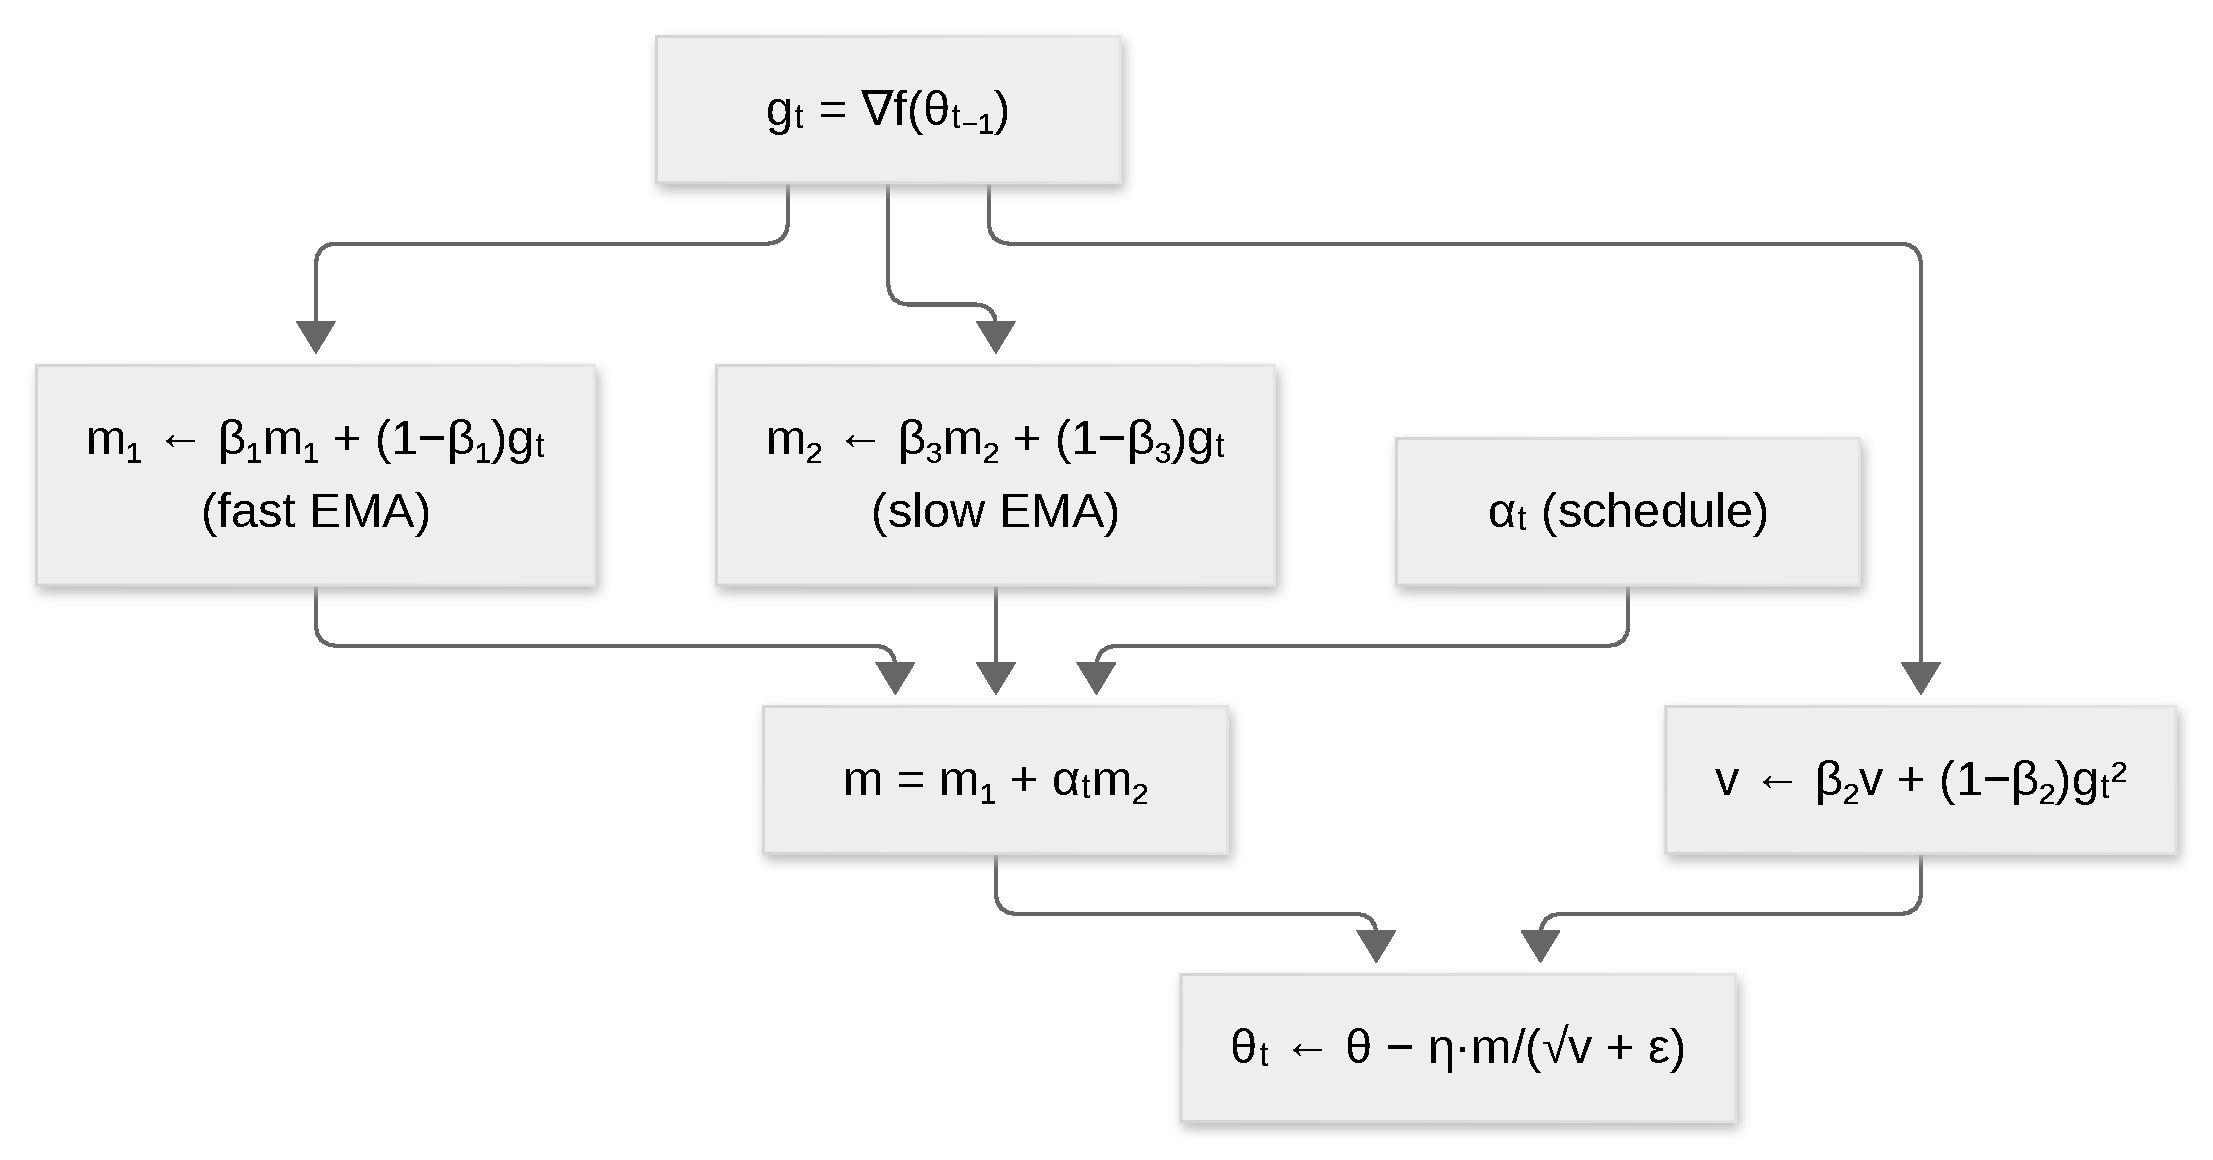
\includegraphics{figures/optimizers/ademamix.pdf}}
\caption{Step flow of AdEMAMix: parallel fast and slow gradient EMAs, mixed with a scheduled weight $\alpha_t$ before the adaptive update.}
\label{fig:opt-ademamix}
\end{figure}
AdEMAMix replaces Adam's single EMA of gradients with a \textbf{mixture of two EMAs}: one fast-decaying and one slow-decaying. This addresses the observation that gradients remain informative over tens of thousands of steps, not just hundreds:
\begin{align}
m_{1,t} &= \beta_1 m_{1,t-1} + (1-\beta_1)g_t \quad\text{(fast EMA, $\beta_1 \approx 0.9$)} \\
m_{2,t} &= \beta_3 m_{2,t-1} + (1-\beta_3)g_t \quad\text{(slow EMA, $\beta_3 \approx 0.9999$)} \\
v_t &= \beta_2 v_{t-1} + (1-\beta_2)g_t^2 \\
m_t &= m_{1,t} + \alpha_t m_{2,t} \quad\text{(mixture with scheduled weight $\alpha_t$)} \\
\theta_{t+1} &= \theta_t - \eta\frac{m_t}{\sqrt{v_t}+\epsilon}
\end{align}
The mixture weight $\alpha_t$ typically increases during training, allowing the fast EMA to provide immediate adaptation while the slow EMA accumulates long-range gradient correlations.

\begin{algorithm}[H]
\caption{AdEMAMix (Exponential Moving Average Mixture)}
\label{alg:ademamix}
\begin{algorithmic}[1]
\Require Initial parameters $\theta_0$, learning rate $\eta$, $\beta_1$ (fast), $\beta_3$ (slow), $\beta_2$ (second moment)
\Require Mixture weight $\alpha_t$ (typically increasing), tolerance $\epsilon$
\Ensure Updated parameters $\theta_T$
\State Initialize: $m_1 \gets 0$ (fast EMA), $m_2 \gets 0$ (slow EMA), $v \gets 0$
\For{$t = 1, 2, \ldots, T$}
    \State $g_t \gets \nabla f(\theta_{t-1})$
    \If{weight\_decay $> 0$}
        \State $\theta_{t-1} \gets \theta_{t-1}(1 - \eta\lambda)$
    \EndIf
    \State $m_1 \gets \beta_1 m_1 + (1-\beta_1) g_t$ \Comment{Fast EMA}
    \State $m_2 \gets \beta_3 m_2 + (1-\beta_3) g_t$ \Comment{Slow EMA}
    \State $v \gets \beta_2 v + (1-\beta_2) g_t^2$
    \State $m_t \gets m_1 + \alpha_t m_2$ \Comment{Mixture}
    \State $\theta_t \gets \theta_{t-1} - \eta (m_t / (\sqrt{v} + \epsilon))$
\EndFor
\Return $\theta_T$
\end{algorithmic}
\end{algorithm}

\paragraph{Cons.}
\begin{itemize}[leftmargin=*]
\item Two gradient EMAs plus the second moment roughly triple Adam's optimizer state.
\item The mixture schedule $\alpha_t$ adds a hyperparameter to tune.
\end{itemize}

\paragraph{Pros.}
\begin{itemize}[leftmargin=*]
\item Exploits gradient information that remains informative over tens of thousands of steps.
\item A 1.3B model on 101B tokens matches AdamW on 197B tokens (95\% data-efficiency gain), suggesting reduced forgetting.
\end{itemize}

\paragraph{MARS (Make Adaptive learning Rates Shine).}
\begin{figure}[H]
\centering
\fitfigure{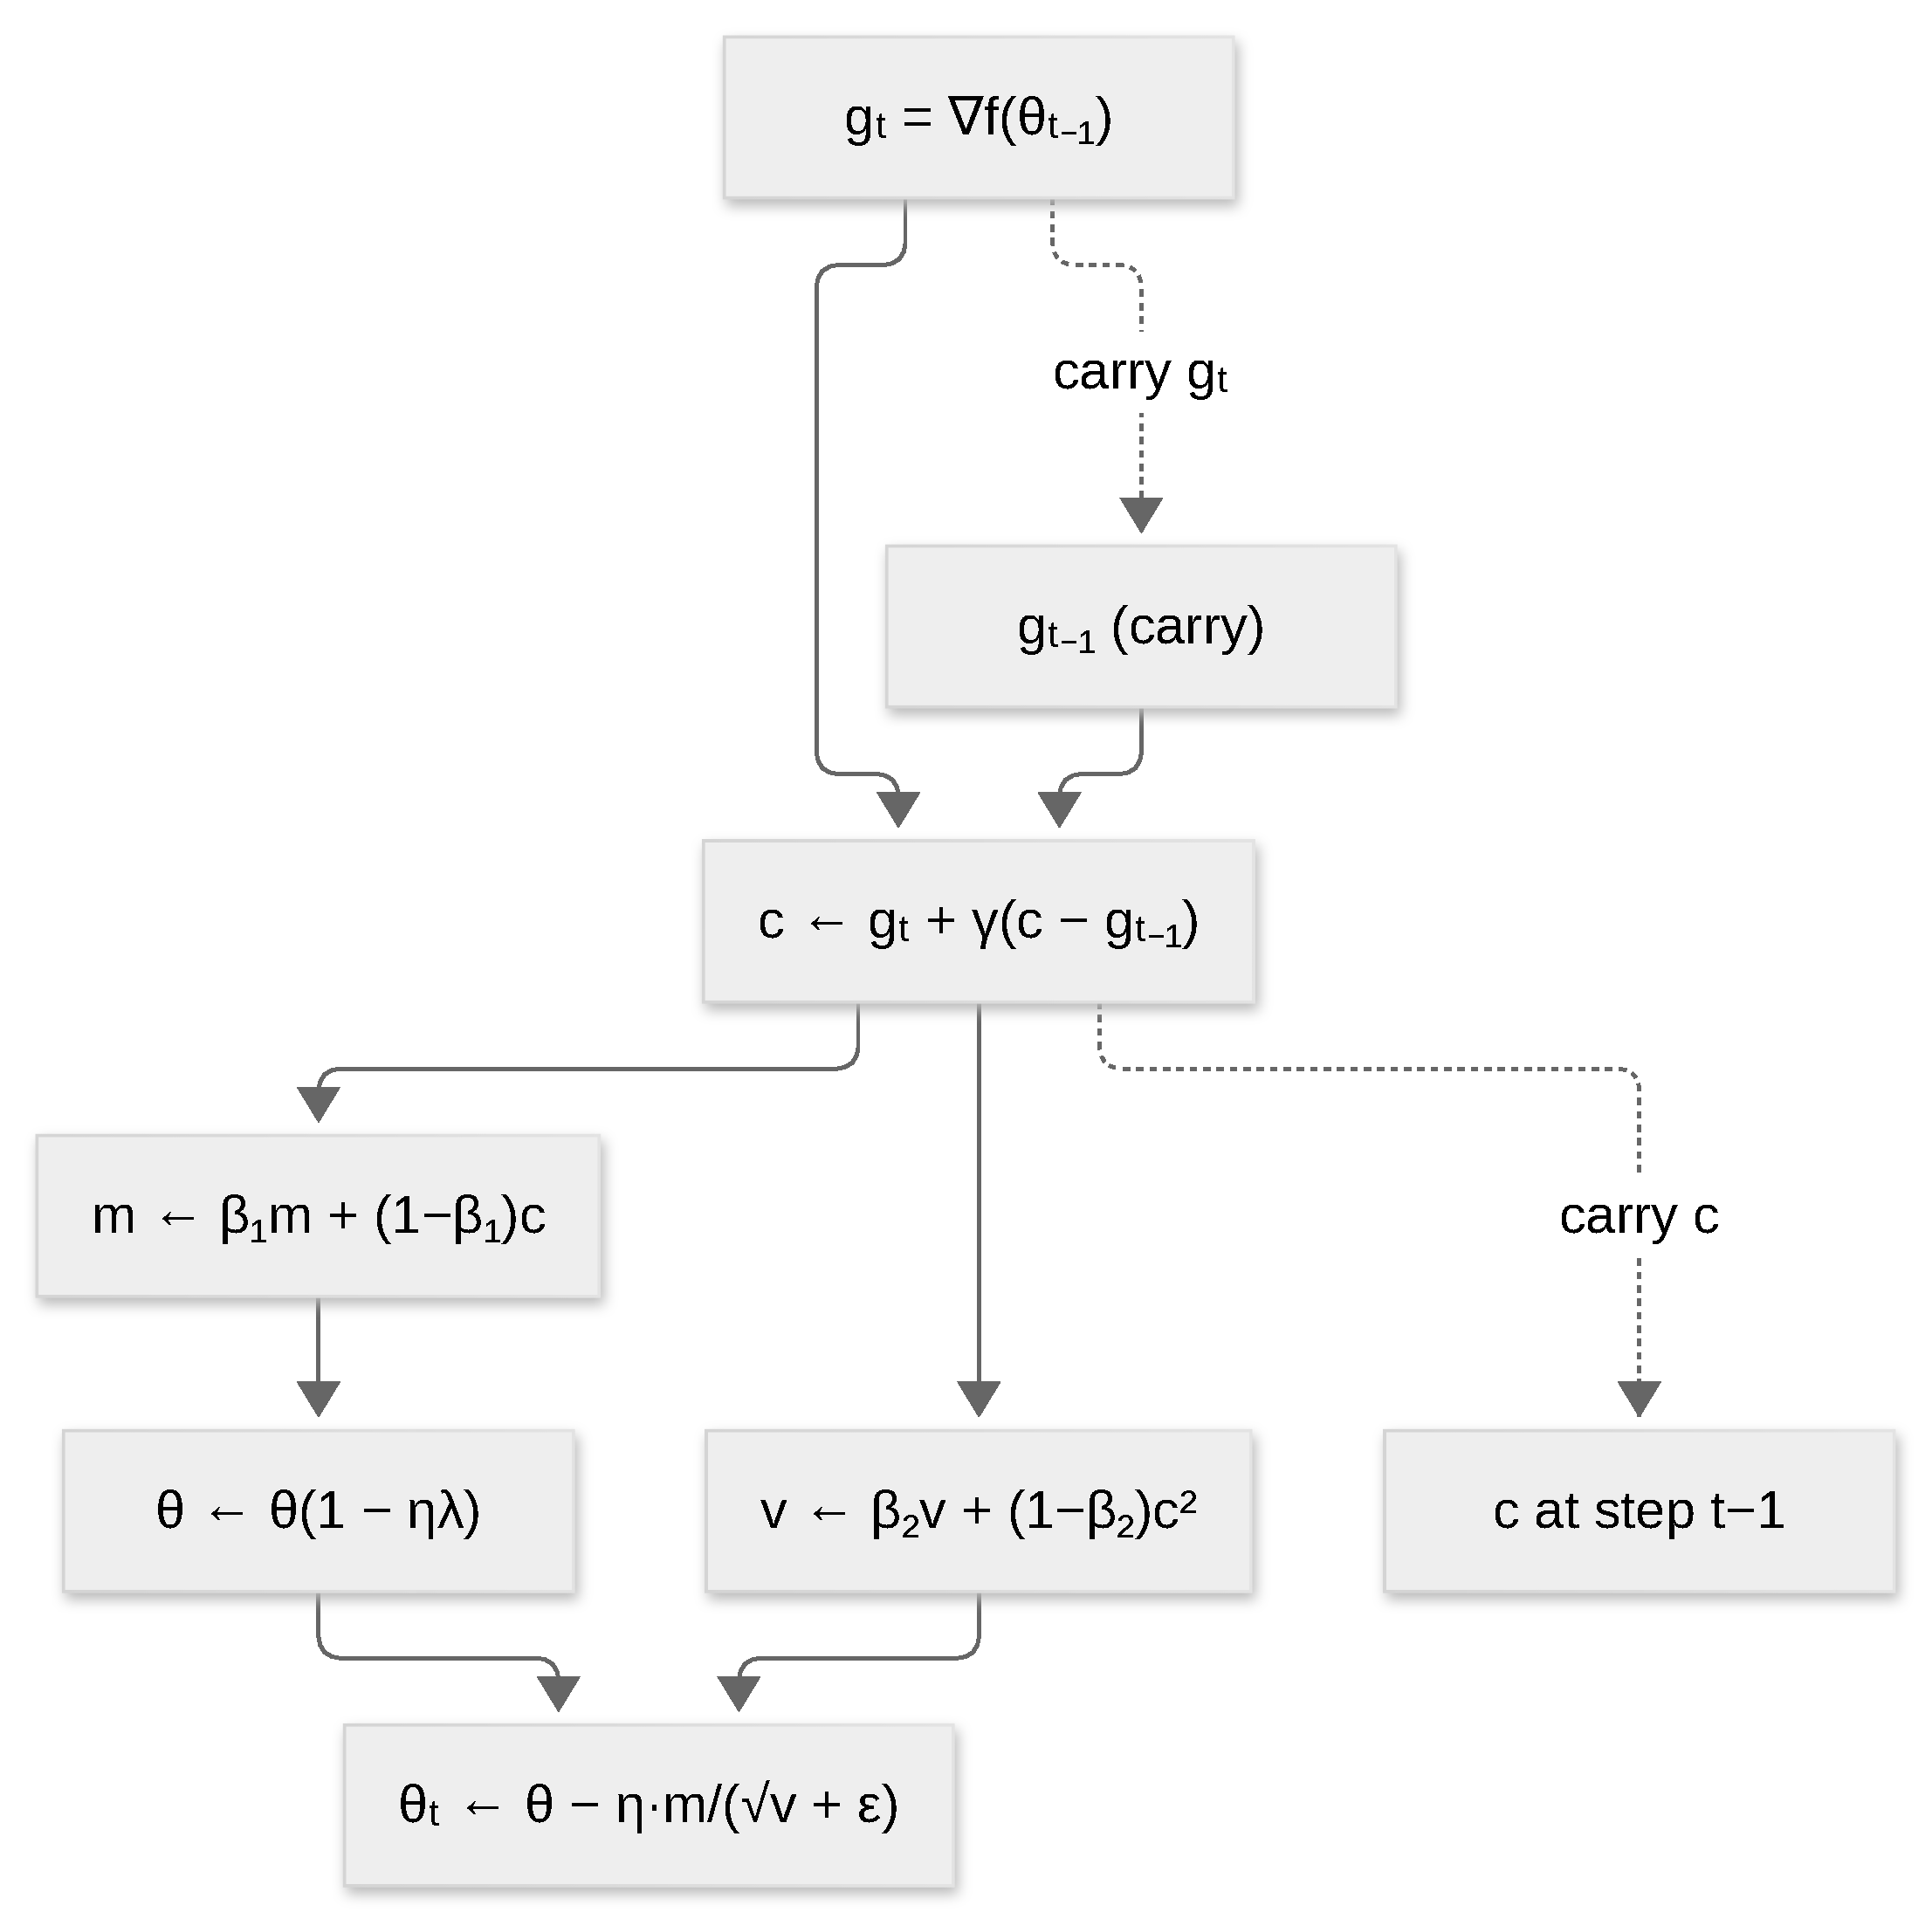
\includegraphics{figures/optimizers/mars.pdf}}
\caption{Step flow of MARS: a recursive variance-reduced gradient estimate feeding Adam-style first and second moments.}
\label{fig:opt-mars}
\end{figure}
MARS combines preconditioned gradient methods (e.g., AdamW) with \textbf{variance reduction} via scaled stochastic recursive momentum. The core innovation is a variance-reduced gradient estimate:
\begin{align}
c_t &= g_t + \gamma(c_{t-1} - g_{t-1}) \quad\text{(SVRG-style recursive estimate)} \\
m_t &= \beta_1 m_{t-1} + (1-\beta_1)c_t \\
v_t &= \beta_2 v_{t-1} + (1-\beta_2)c_t^2 \\
\theta_{t+1} &= \theta_t - \eta\frac{m_t}{\sqrt{v_t}+\epsilon}
\end{align}
where $\gamma \in [0.01, 0.1]$ controls how much historical gradient information is retained. The variance-reduced gradient $c_t$ acts as an implicit noise filter, amplifying consistent signal directions and dampening contradictory noise.

\begin{algorithm}[H]
\caption{MARS (Make Adaptive learning Rates Shine)}
\label{alg:mars}
\begin{algorithmic}[1]
\Require Initial parameters $\theta_0$, learning rate $\eta$, $\beta_1, \beta_2$, weight decay $\lambda$
\Require Variance reduction coefficient $\gamma \in [0.01, 0.1]$
\Ensure Updated parameters $\theta_T$
\State Initialize: $m \gets 0$, $v \gets 0$, $c \gets 0$ (variance-reduced gradient), $g_{-1} \gets 0$
\For{$t = 1, 2, \ldots, T$}
    \State $g_t \gets \nabla f(\theta_{t-1})$
    \State Variance reduction: $c \gets g_t + \gamma(c - g_{t-1})$
    \State $m \gets \beta_1 m + (1-\beta_1) c$
    \State $v \gets \beta_2 v + (1-\beta_2) c^2$
    \If{weight\_decay $> 0$}
        \State $\theta_{t-1} \gets \theta_{t-1}(1 - \eta\lambda)$
    \EndIf
    \State $\theta_t \gets \theta_{t-1} - \eta (m / (\sqrt{v} + \epsilon))$
    \State $g_{t-1} \gets g_t$
\EndFor
\Return $\theta_T$
\end{algorithmic}
\end{algorithm}

\paragraph{Cons.}
\begin{itemize}[leftmargin=*]
\item Stores the variance-reduced gradient and the previous gradient in addition to Adam's moments.
\item The variance-reduction coefficient $\gamma \in [0.01, 0.1]$ must be tuned.
\end{itemize}

\paragraph{Pros.}
\begin{itemize}[leftmargin=*]
\item Acts as an implicit noise filter, amplifying consistent directions and dampening contradictory noise.
\item MARS-AdamW consistently outperforms bare AdamW by significant margins on GPT-2 pretraining.
\end{itemize}

\paragraph{Cautious Optimizers (Cautious AdamW, Cautious Lion).}
\begin{figure}[H]
\centering
\fitfigure{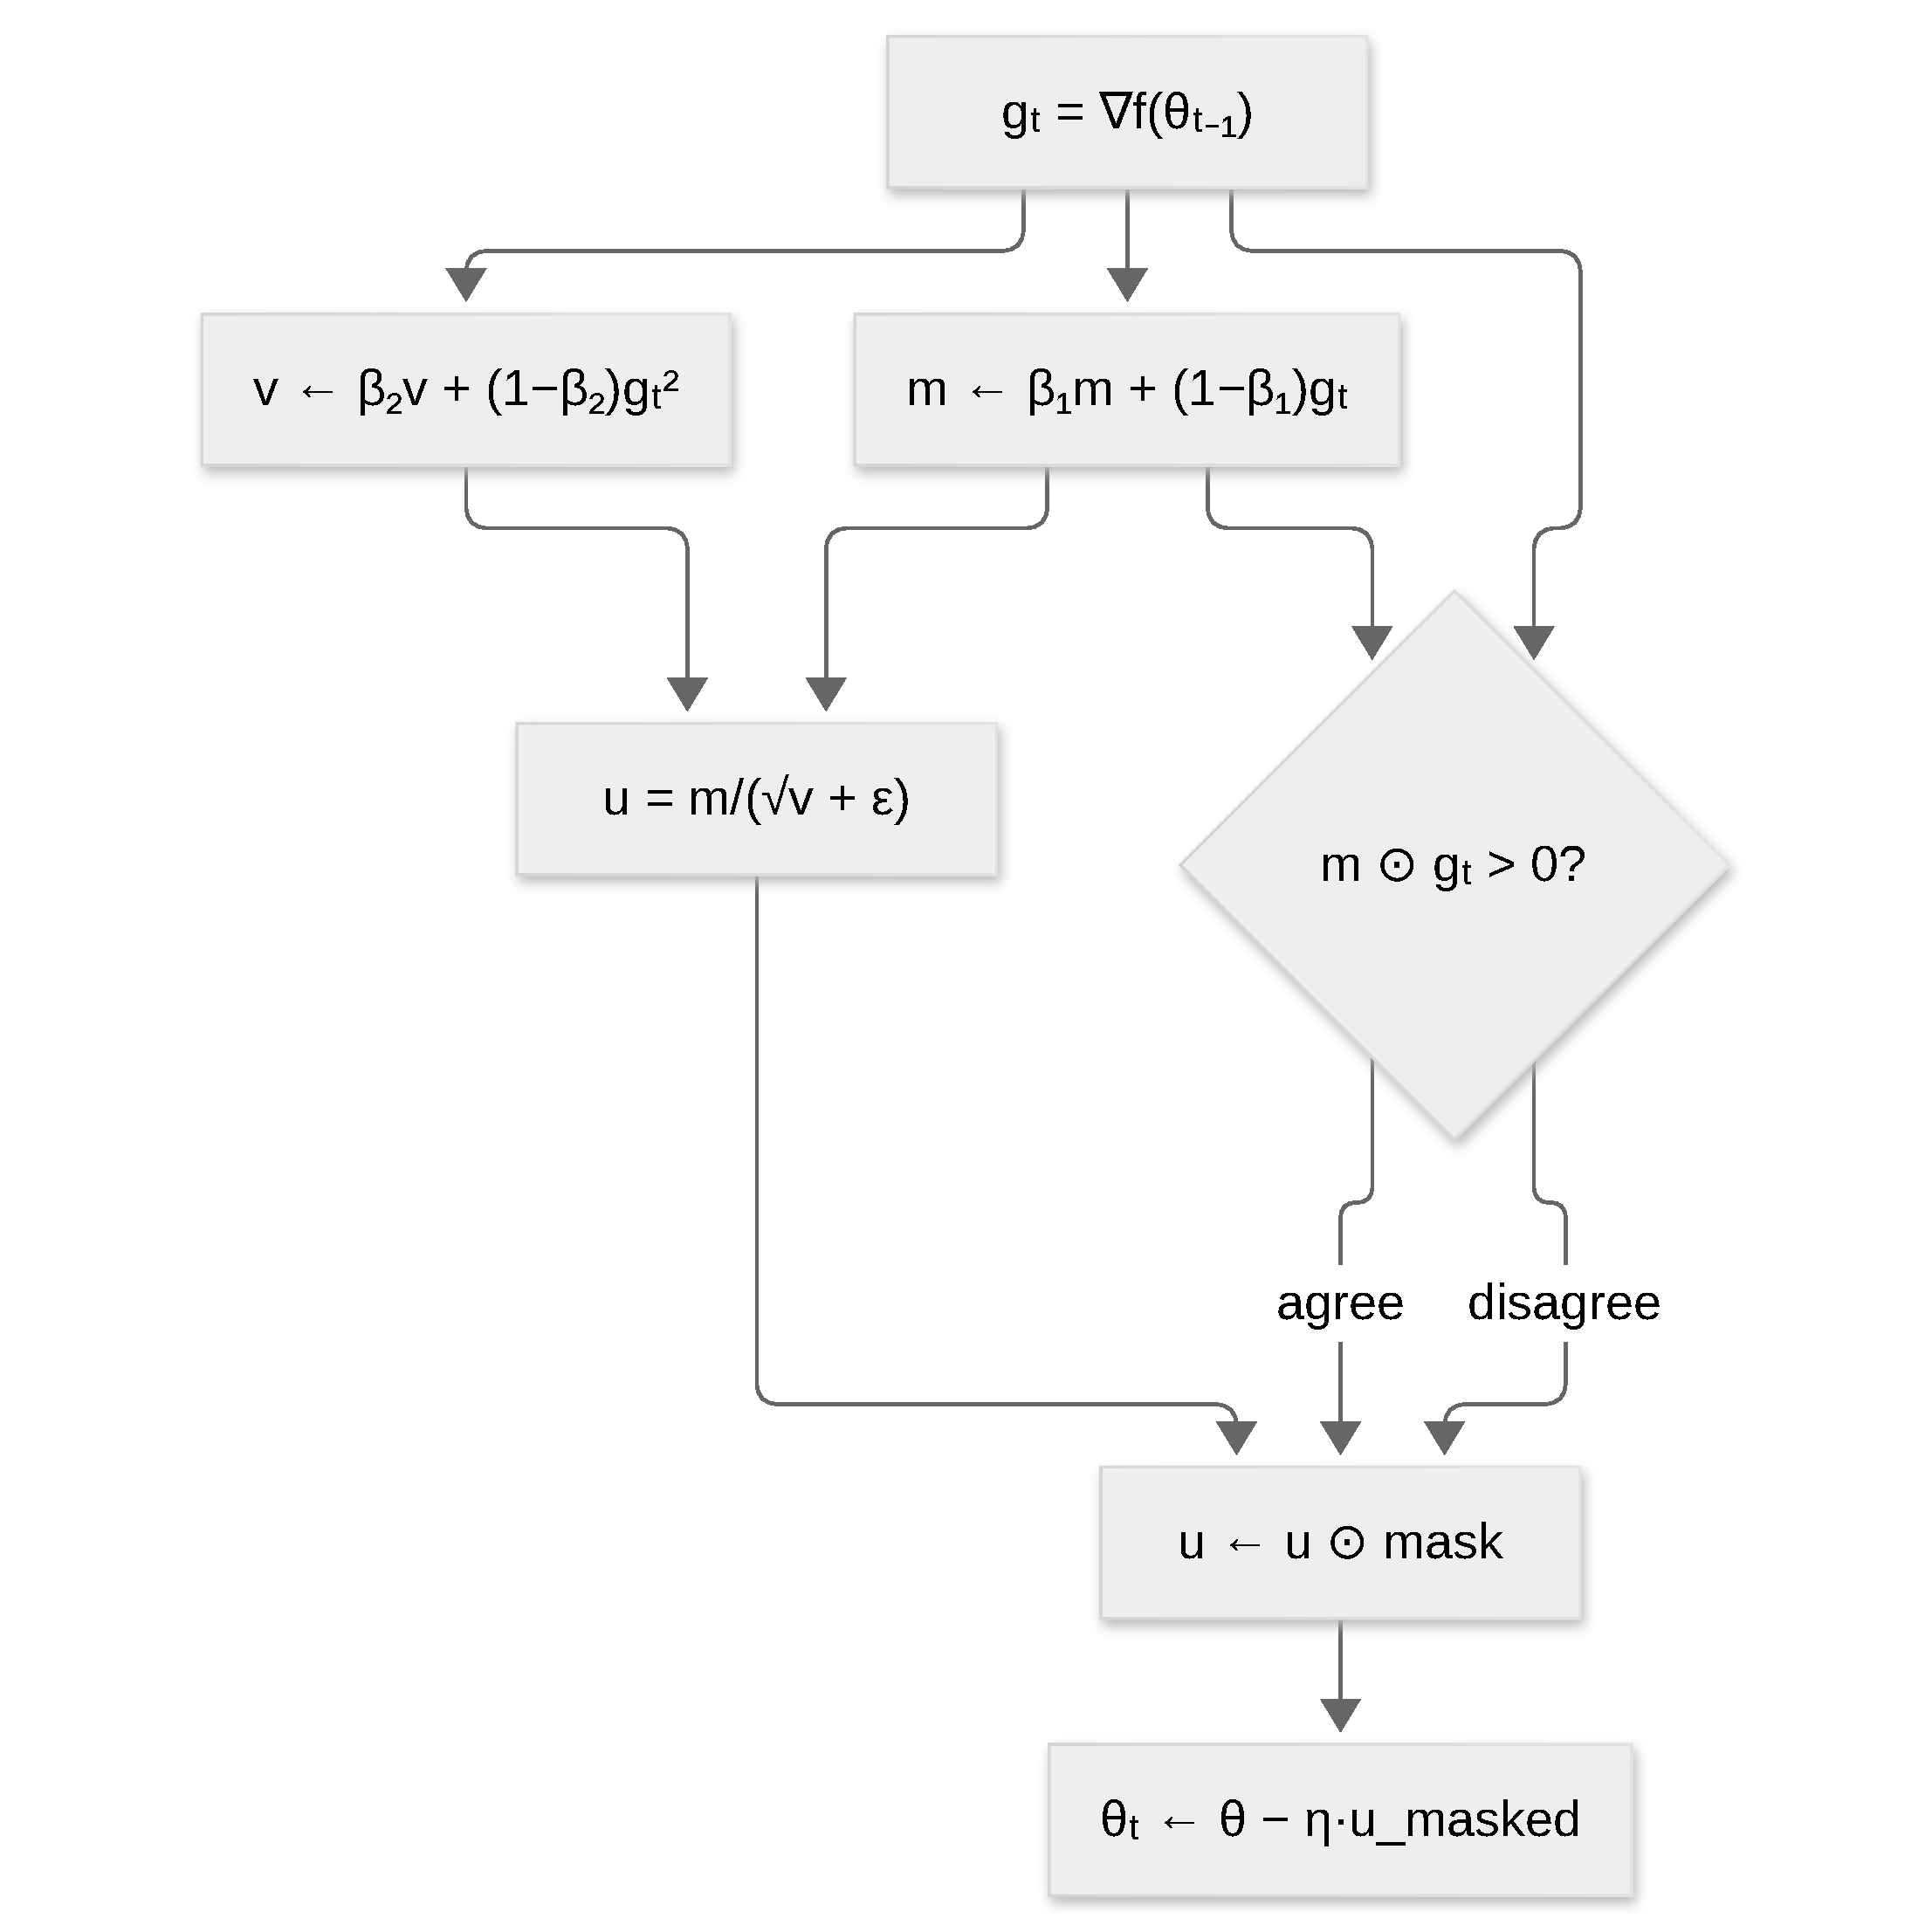
\includegraphics{figures/optimizers/cautious.pdf}}
\caption{Step flow of Cautious AdamW: a consensus mask keeps only update coordinates where momentum and gradient agree.}
\label{fig:opt-cautious}
\end{figure}
The Cautious framework applies a \textbf{one-line modification} to any momentum-based optimizer: mask the update so that only dimensions where momentum and gradient directions agree are applied:
\begin{align}
\text{mask}_i &= \begin{cases} 1 & \text{if } m_t[i] \cdot g_t[i] > 0 \quad\text{(agreement)} \\ 0 & \text{otherwise} \end{cases} \\
u_t &= \left(\frac{m_t}{\sqrt{v_t}+\epsilon}\right) \odot \text{mask} \quad\text{(element-wise masking)} \\
\theta_{t+1} &= \theta_t - \eta u_t
\end{align}
The intuition: momentum $m_t$ estimates the gradient direction from history; the current gradient $g_t$ is instantaneous signal. When both agree, the optimizer is confident and should update aggressively. When they disagree, the optimizer is conflicted---the historical trend points toward a region that may have been good before, but current evidence contradicts it. By masking conflicted dimensions, Cautious becomes more conservative and avoids corrupted steps.

\begin{algorithm}[H]
\caption{Cautious AdamW (Consensus-based Update Masking)}
\label{alg:cautious}
\begin{algorithmic}[1]
\Require Initial parameters $\theta_0$, learning rate $\eta$, $\beta_1, \beta_2$, weight decay $\lambda$
\Ensure Updated parameters $\theta_T$
\State Initialize: $m \gets 0$, $v \gets 0$
\For{$t = 1, 2, \ldots, T$}
    \State $g_t \gets \nabla f(\theta_{t-1})$
    \State $m \gets \beta_1 m + (1-\beta_1) g_t$
    \State $v \gets \beta_2 v + (1-\beta_2) g_t^2$
    \State Consensus mask: $\text{mask}_i \gets 1$ if $m[i] \cdot g_t[i] > 0$, else $0$ \Comment{Agreement}
    \State Base Adam update: $u \gets m / (\sqrt{v} + \epsilon)$
    \State Apply mask: $u_{\text{masked}} \gets u \odot \text{mask}$ \Comment{Element-wise}
    \If{weight\_decay $> 0$}
        \State $\theta_{t-1} \gets \theta_{t-1}(1 - \eta\lambda)$
    \EndIf
    \State $\theta_t \gets \theta_{t-1} - \eta u_{\text{masked}}$
\EndFor
\Return $\theta_T$
\end{algorithmic}
\end{algorithm}

\paragraph{Cons.}
\begin{itemize}[leftmargin=*]
\item Masking can discard useful updates when momentum and gradient temporarily disagree.
\item Requires a base momentum optimizer plus the element-wise mask.
\end{itemize}

\paragraph{Pros.}
\begin{itemize}[leftmargin=*]
\item A one-line modification applicable to any momentum-based optimizer.
\item Up to \textbf{1.47$\times$ speedup} on Llama and MAE pretraining while preserving convergence guarantees.
\end{itemize}

